\protect\newpage
\begin{center}
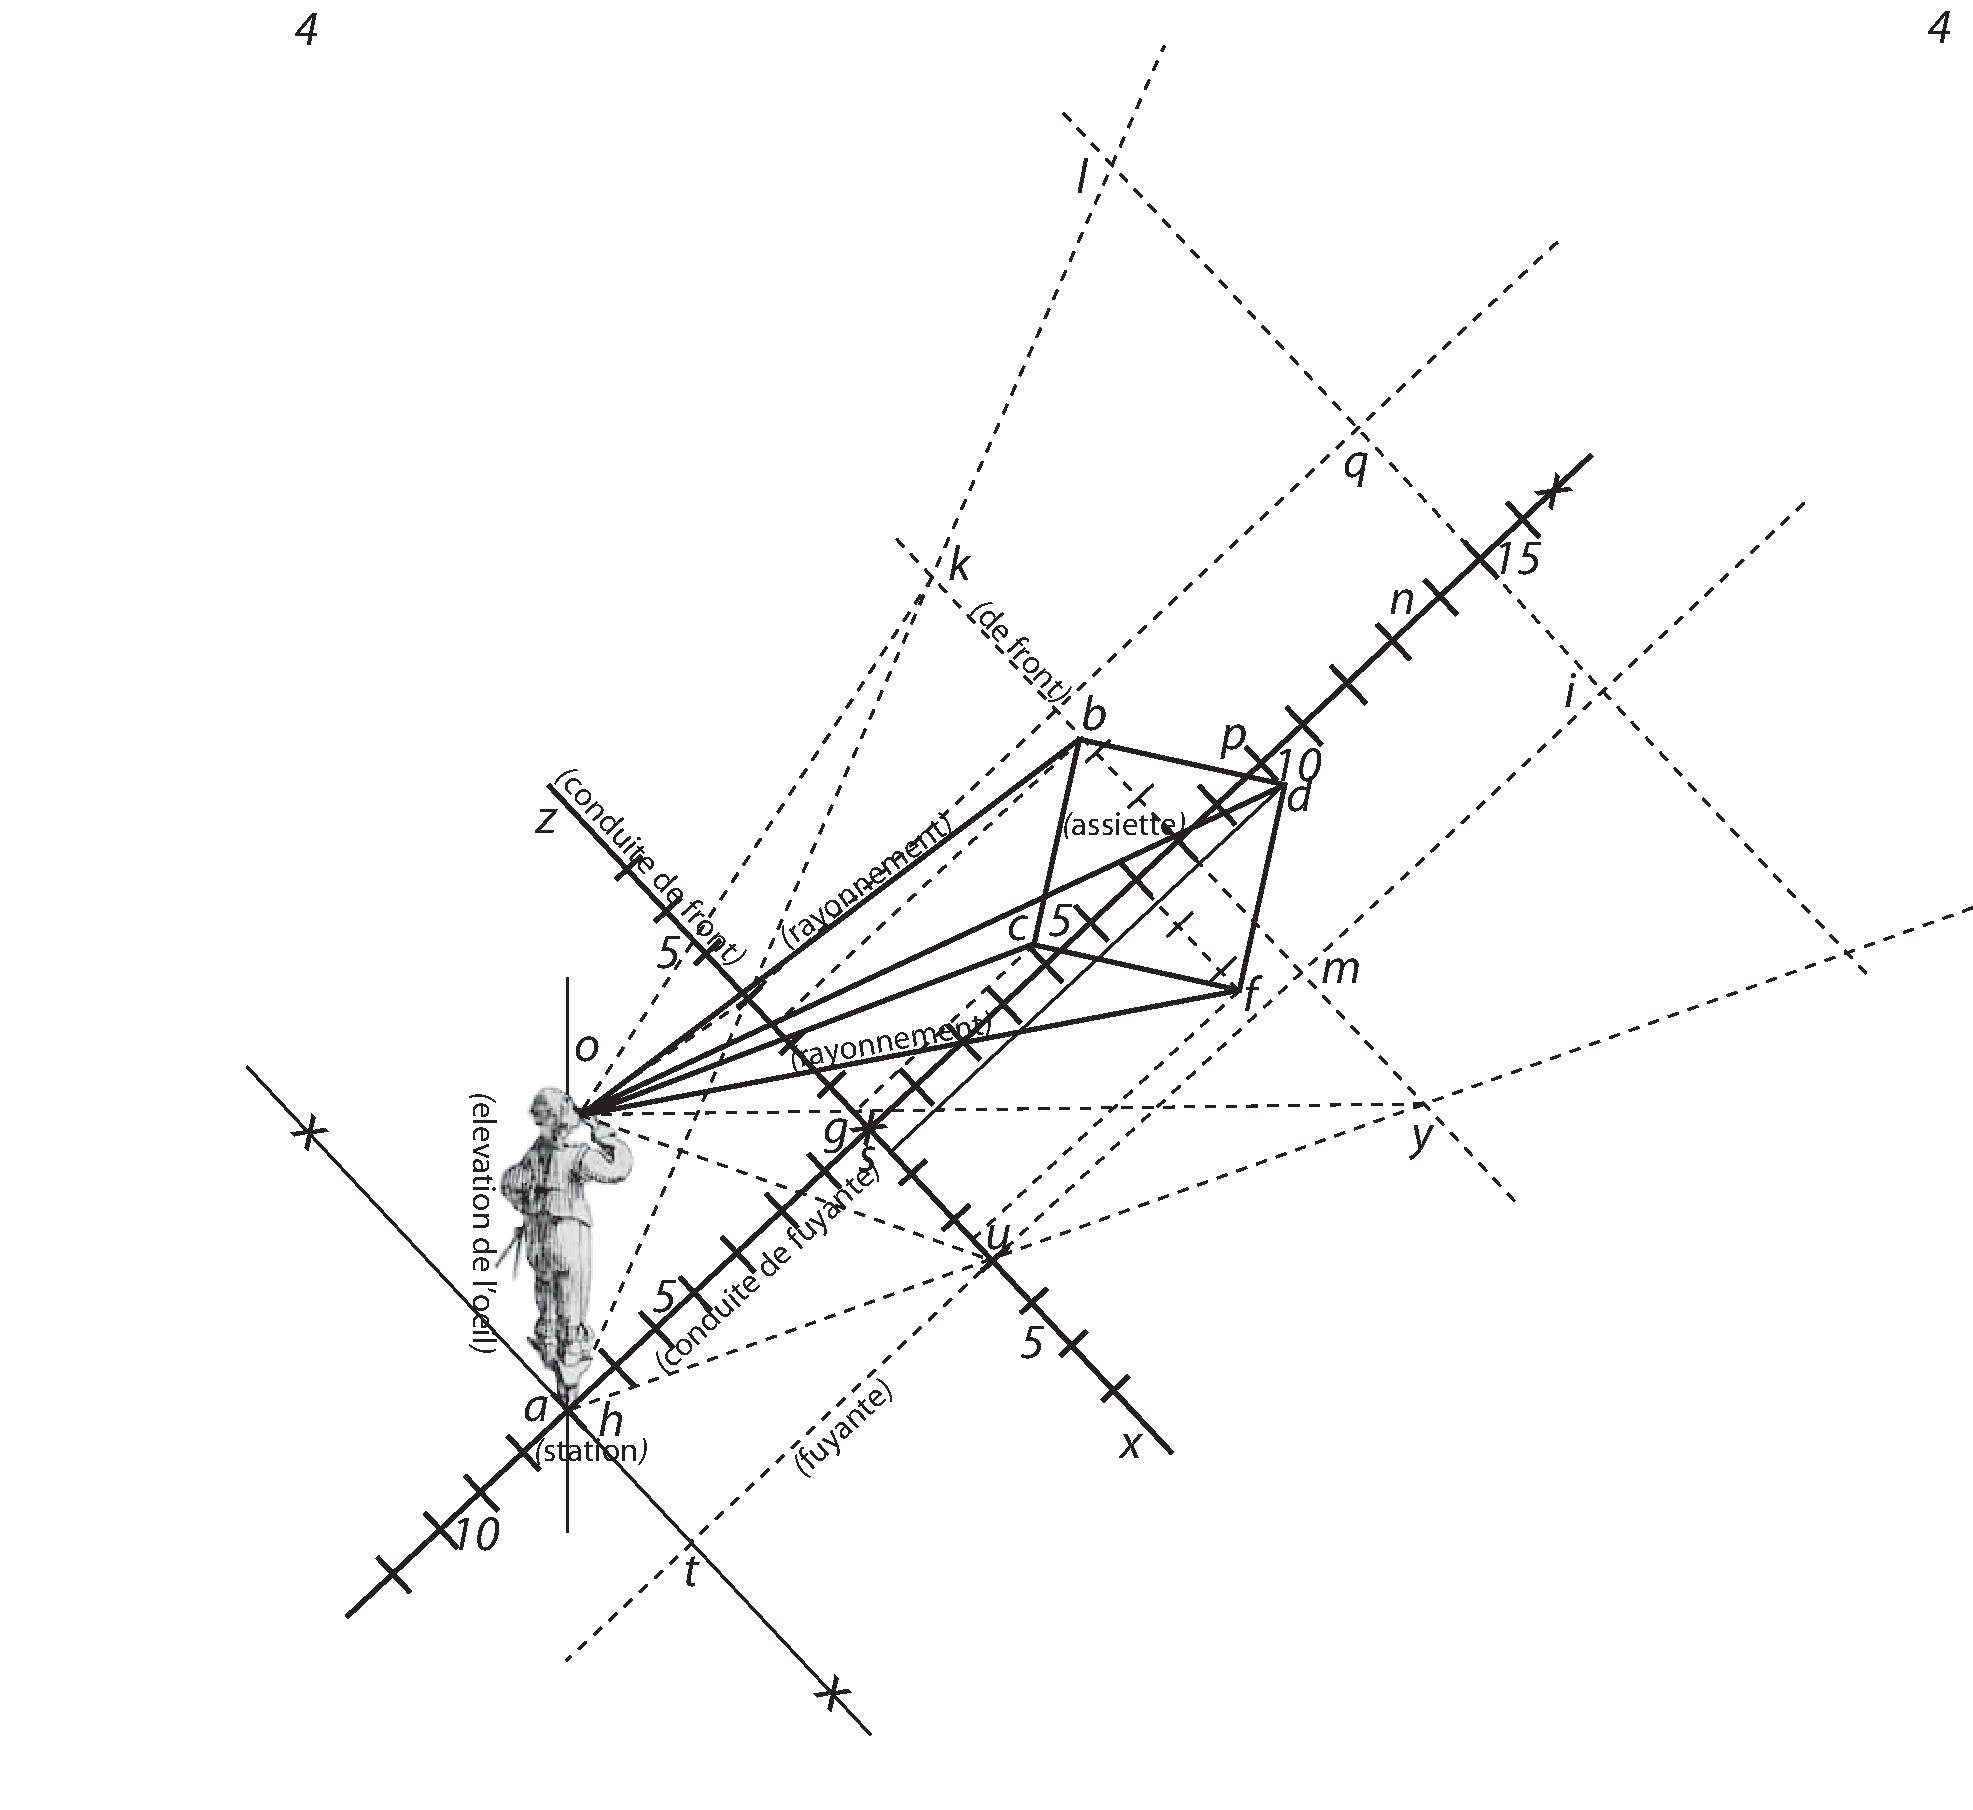
\includegraphics[width=1.0\textwidth]{images/T4-Desargues}
\\\rule[-4mm]{0mm}{10mm}\textit{[Fig. 1]}
\protect\newpage
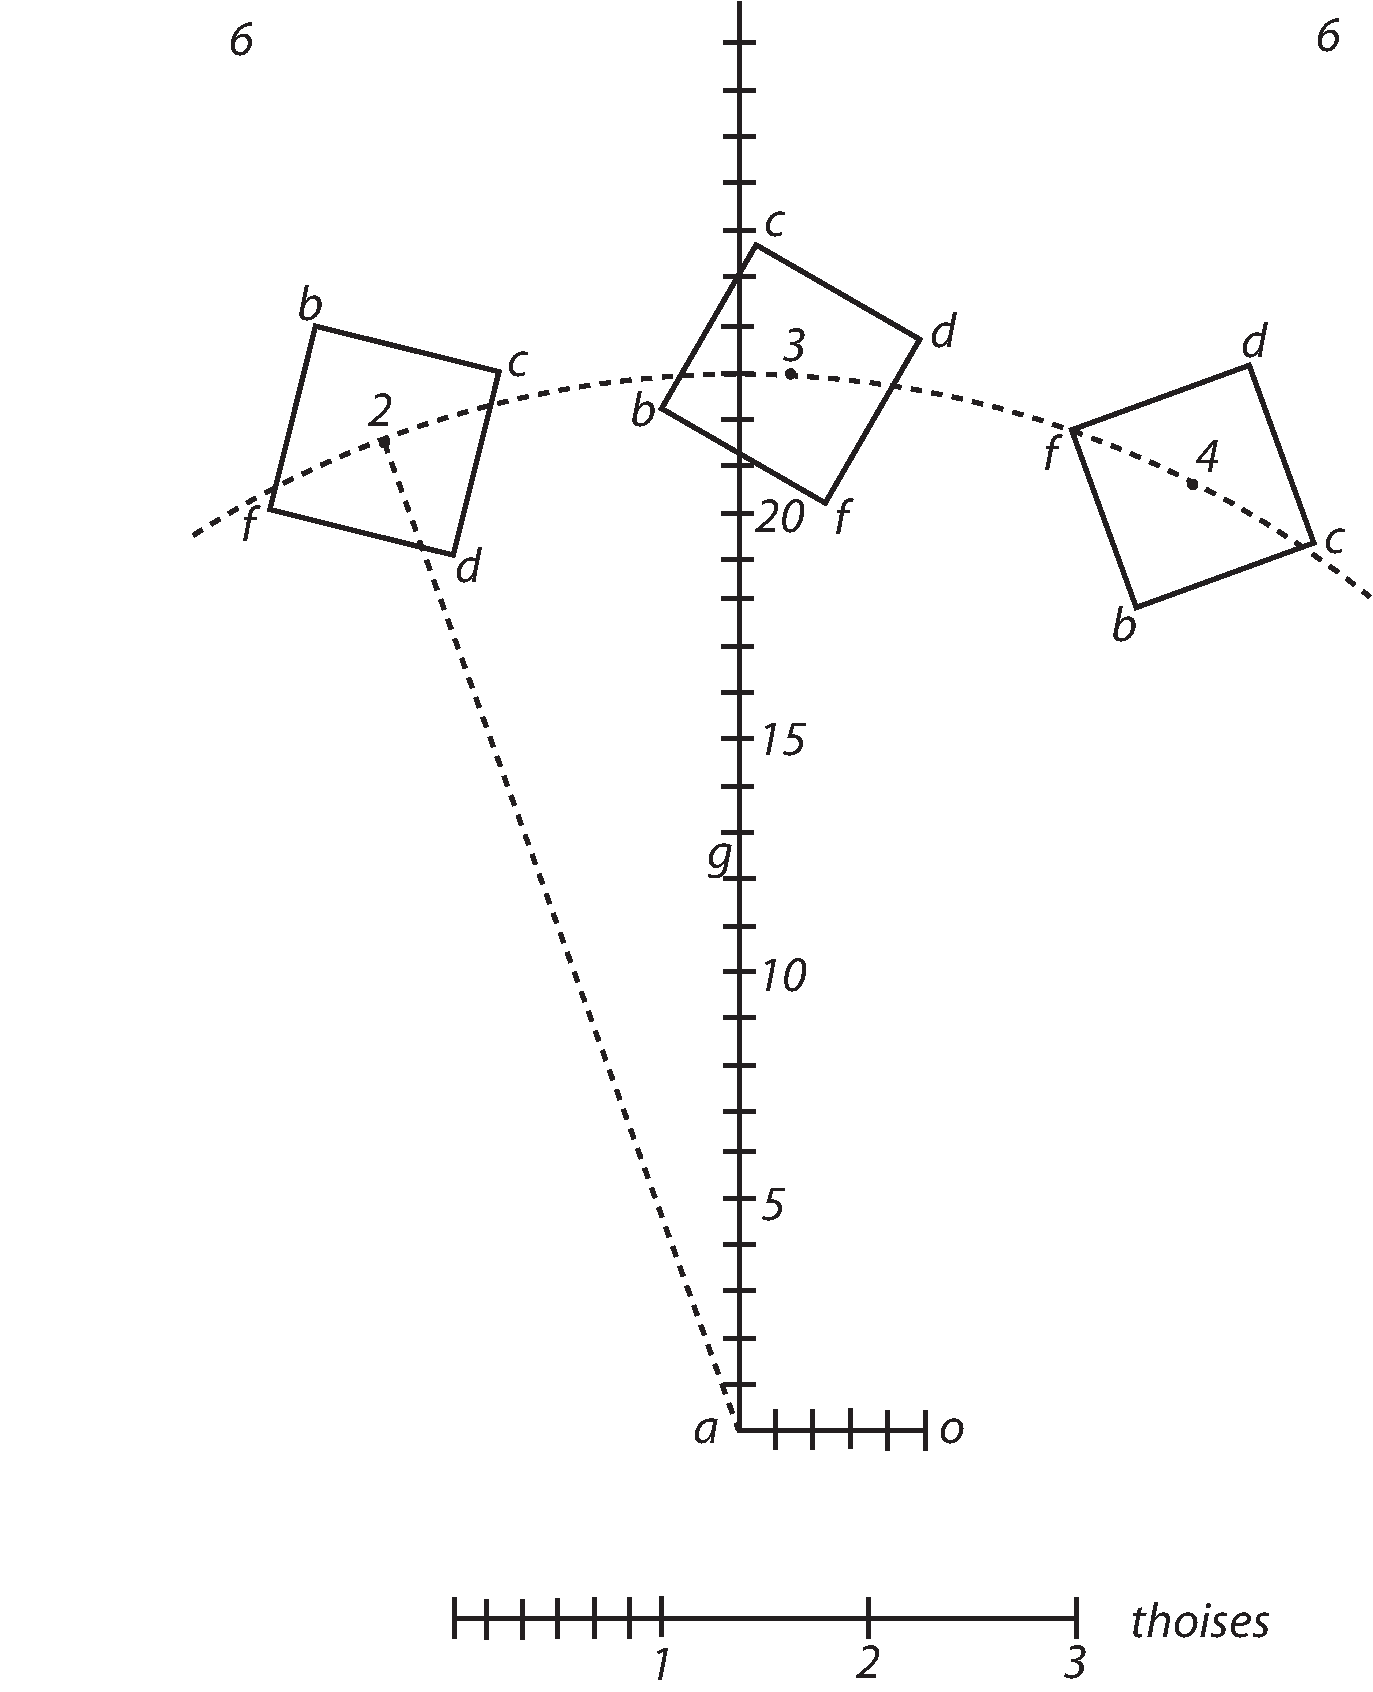
\includegraphics[width=0.7\textwidth]{images/T6-Desargues}
\\\rule[-4mm]{0mm}{10mm}\textit{[Fig. 2]}
\footnote{\textit{Im mittleren Teil der Zeichnung links}: la 4\textsuperscript{me} planche commence les nombres par \textit{g}}
\protect\newpage
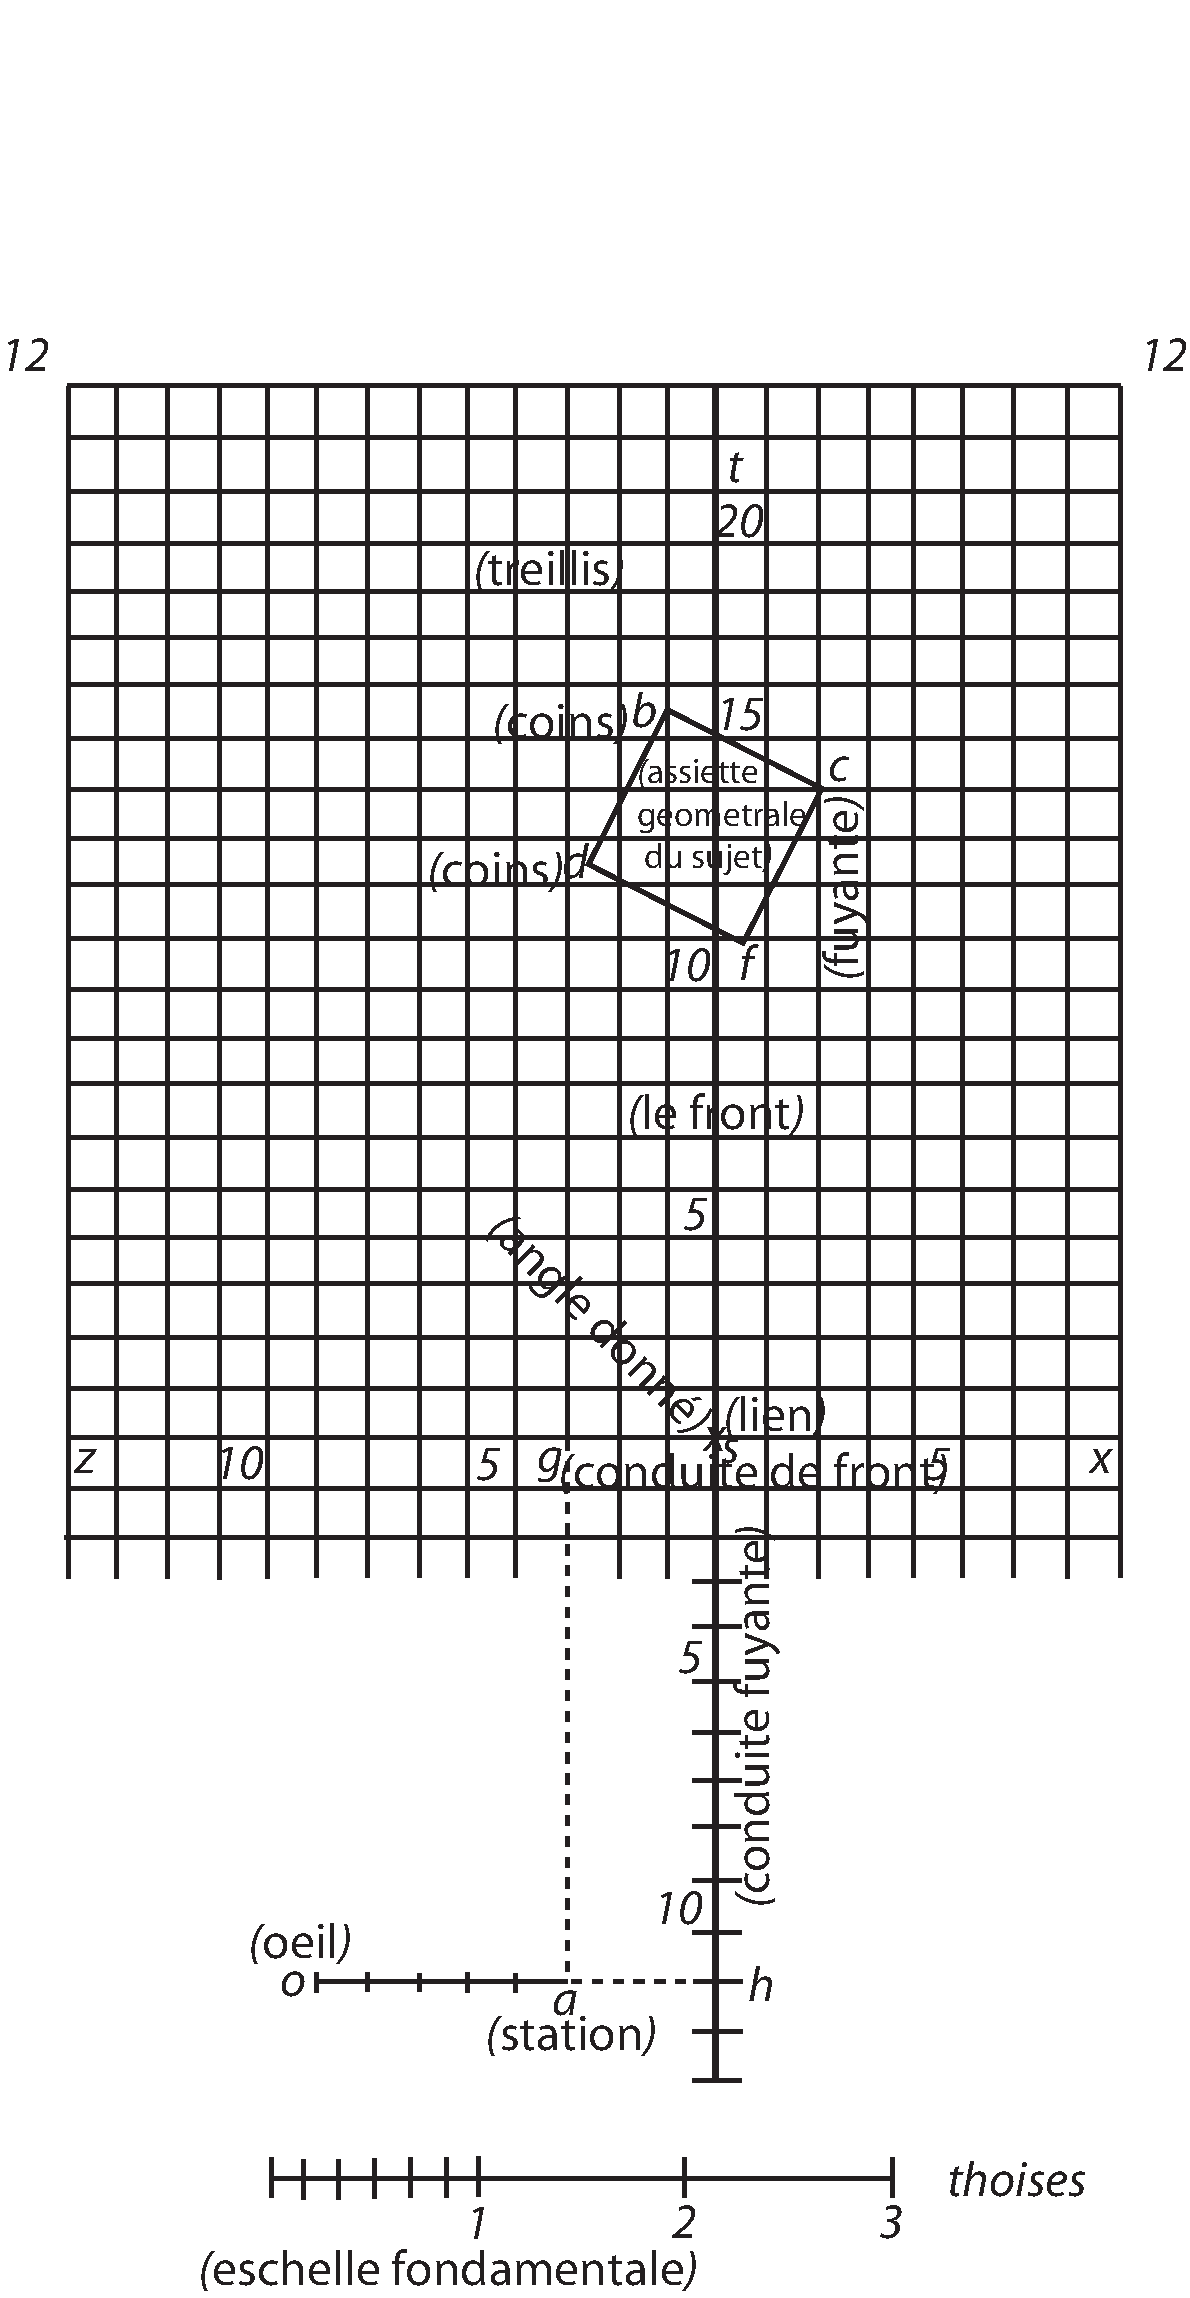
\includegraphics[width=0.7\textwidth]{images/T12-Desargues}
\\\textit{[Fig. 4]}
\protect\newpage
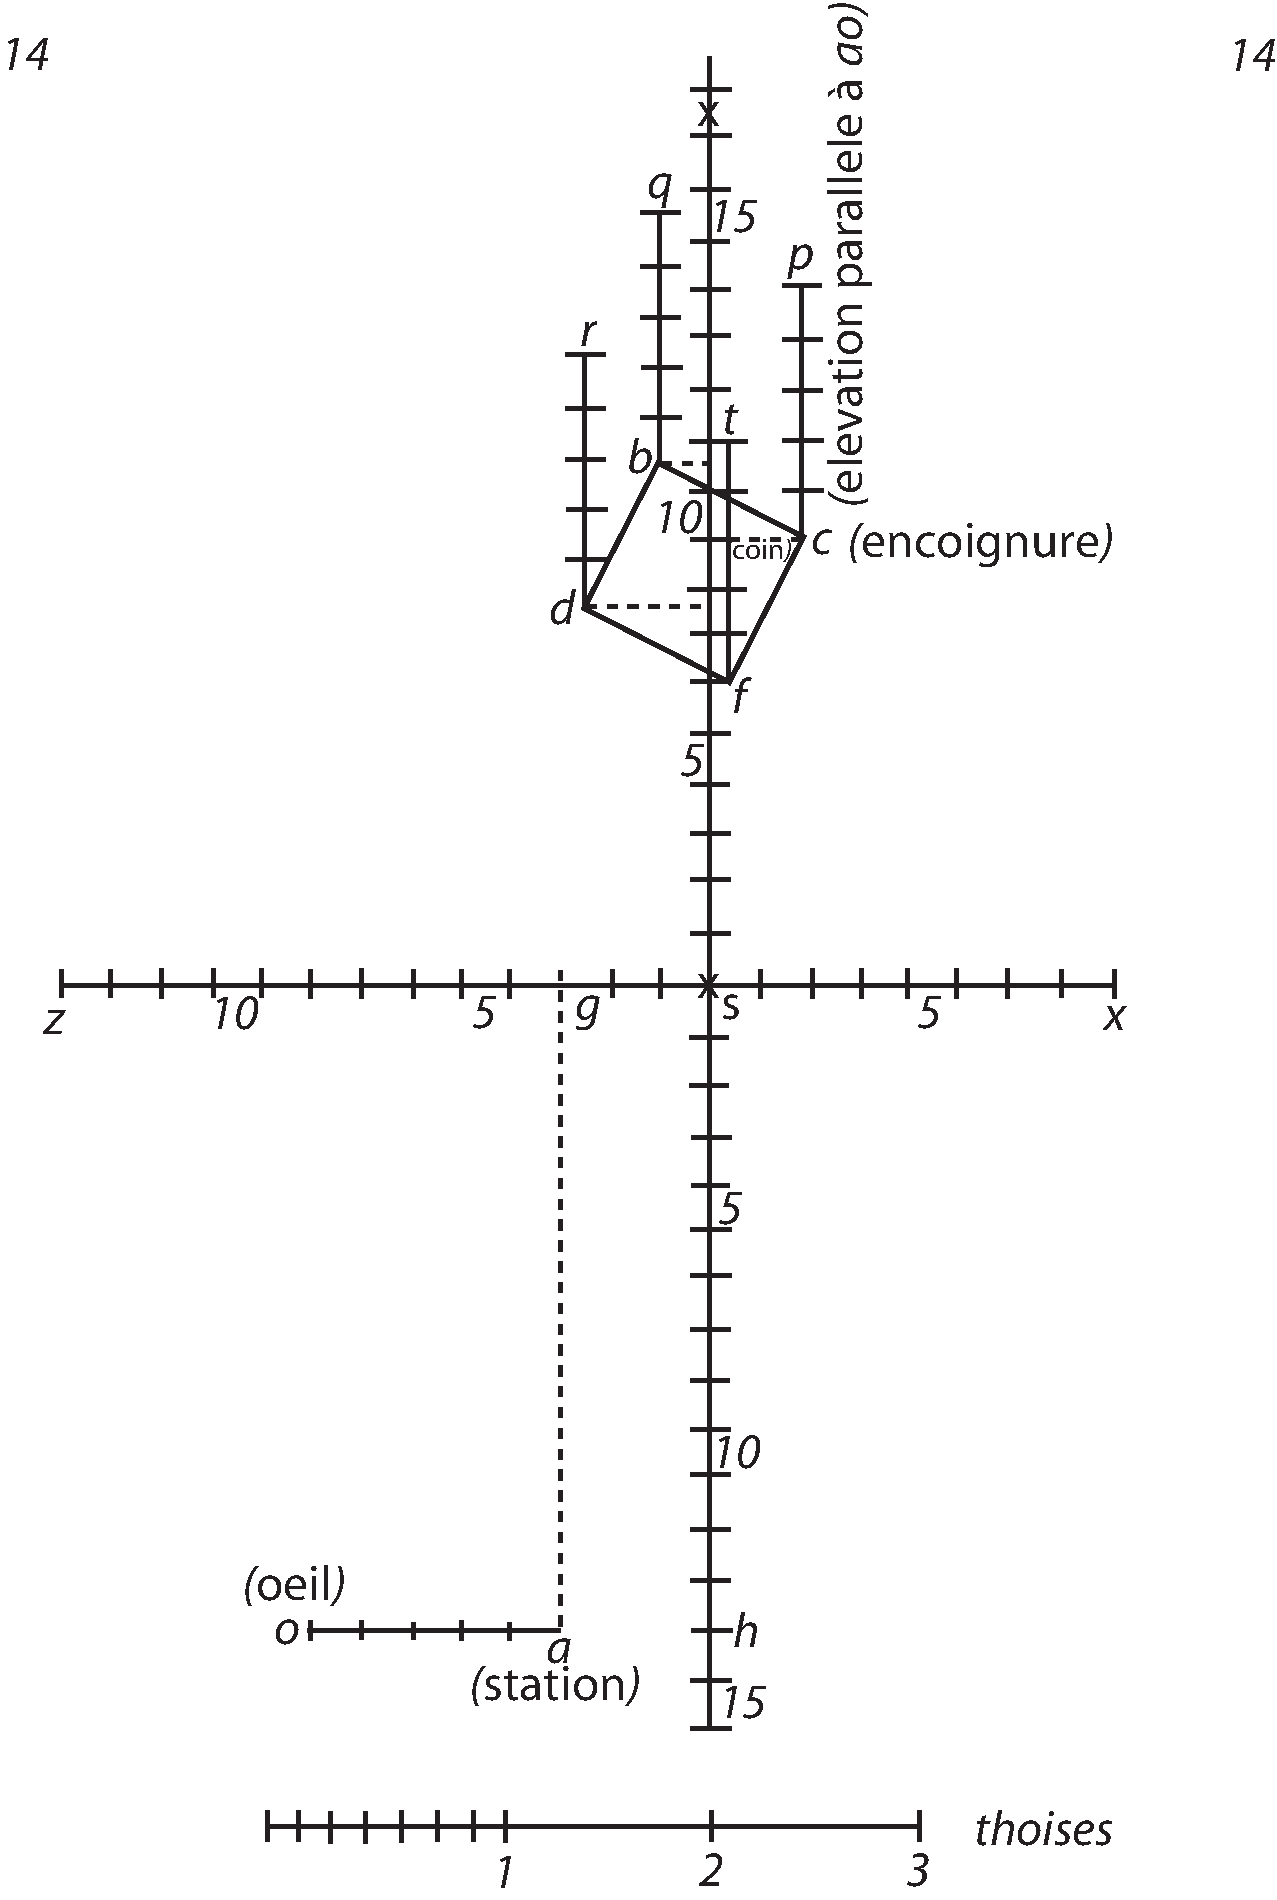
\includegraphics[width=0.78\textwidth]{images/T14-Desargues}
\\\rule[-4mm]{0mm}{10mm}\textit{[Fig. 5]}
\protect\newpage
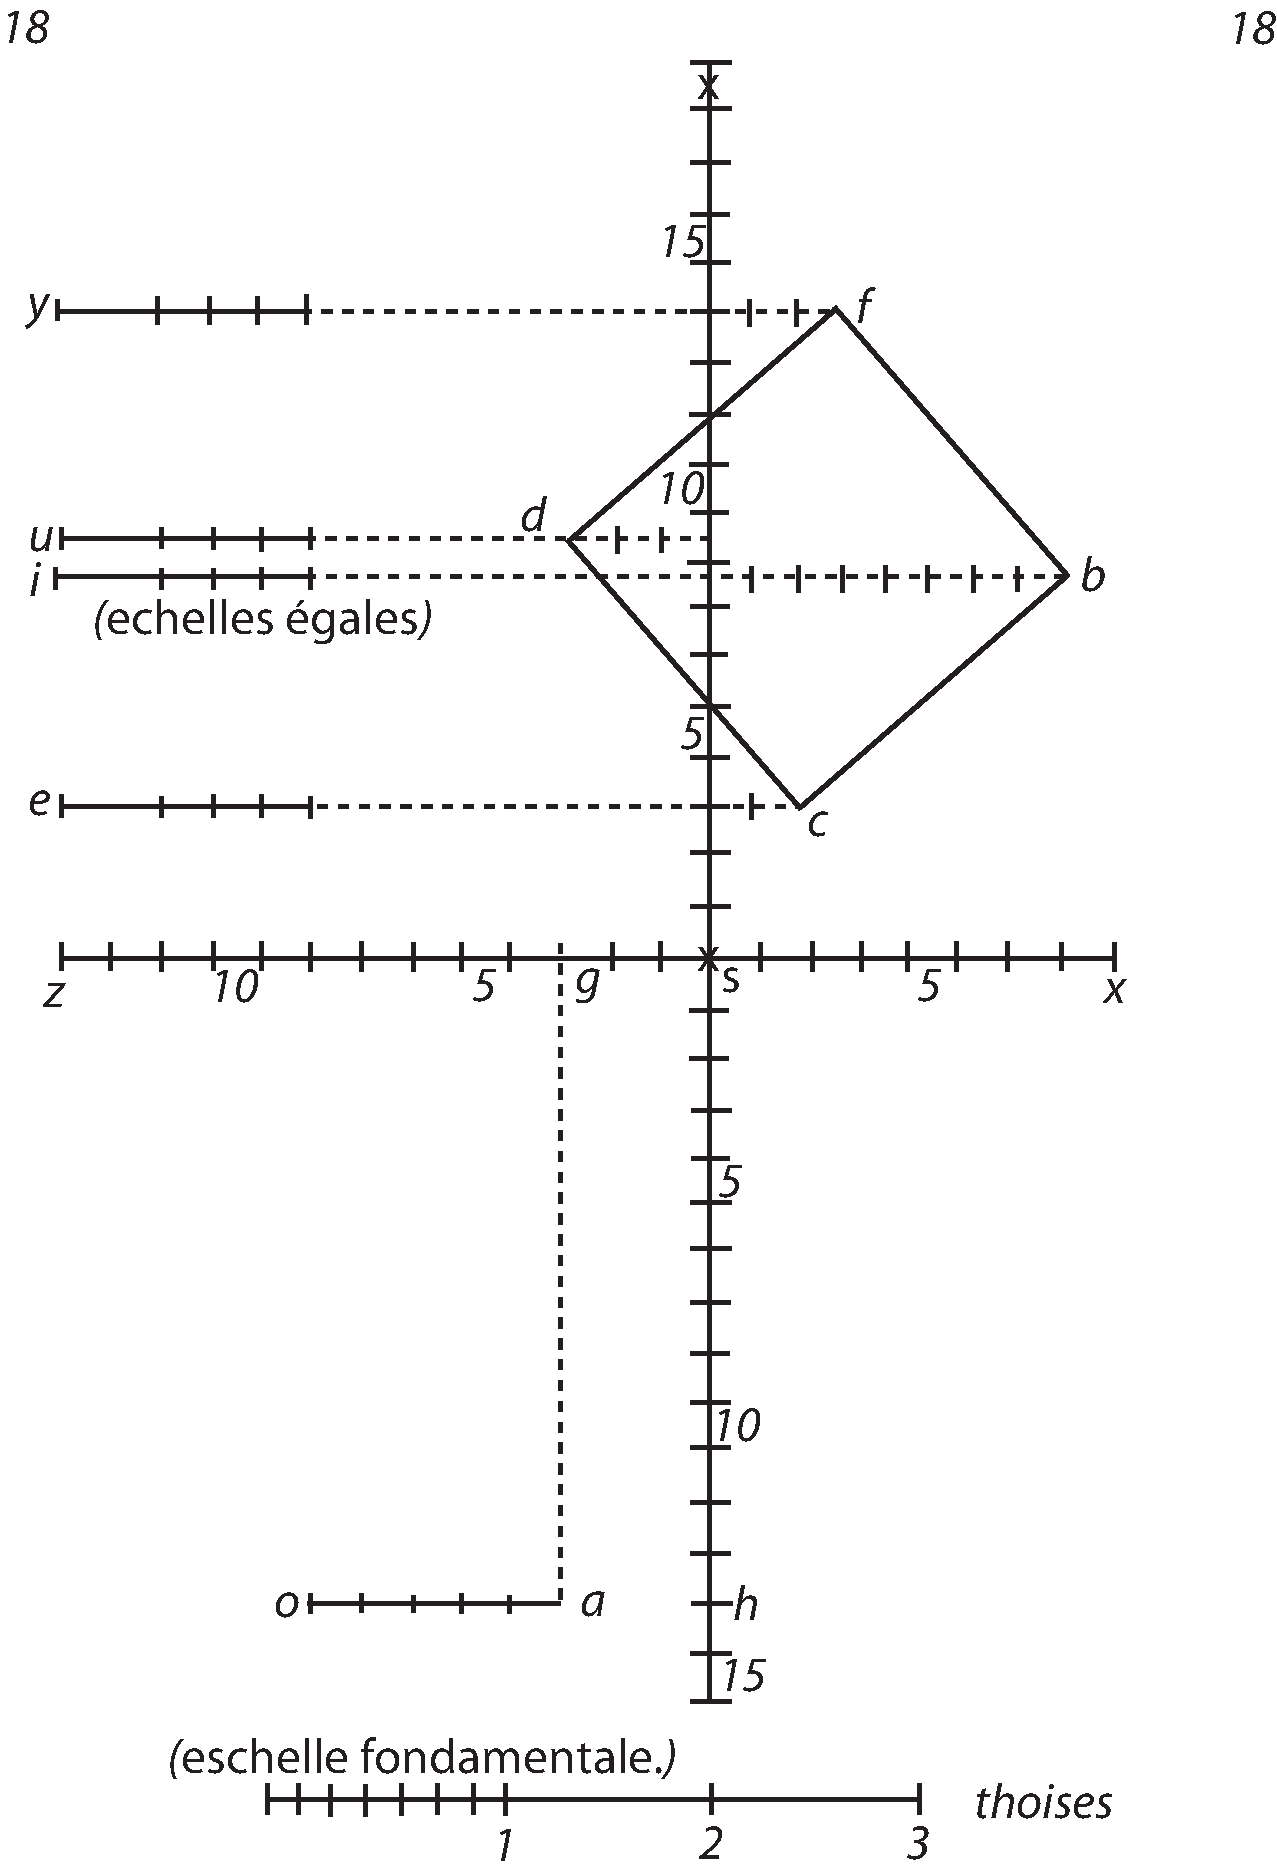
\includegraphics[width=0.7\textwidth]{images/T18-Desargues}
\\\rule[-4mm]{0mm}{10mm}\textit{[Fig. 6]}
\protect\newpage
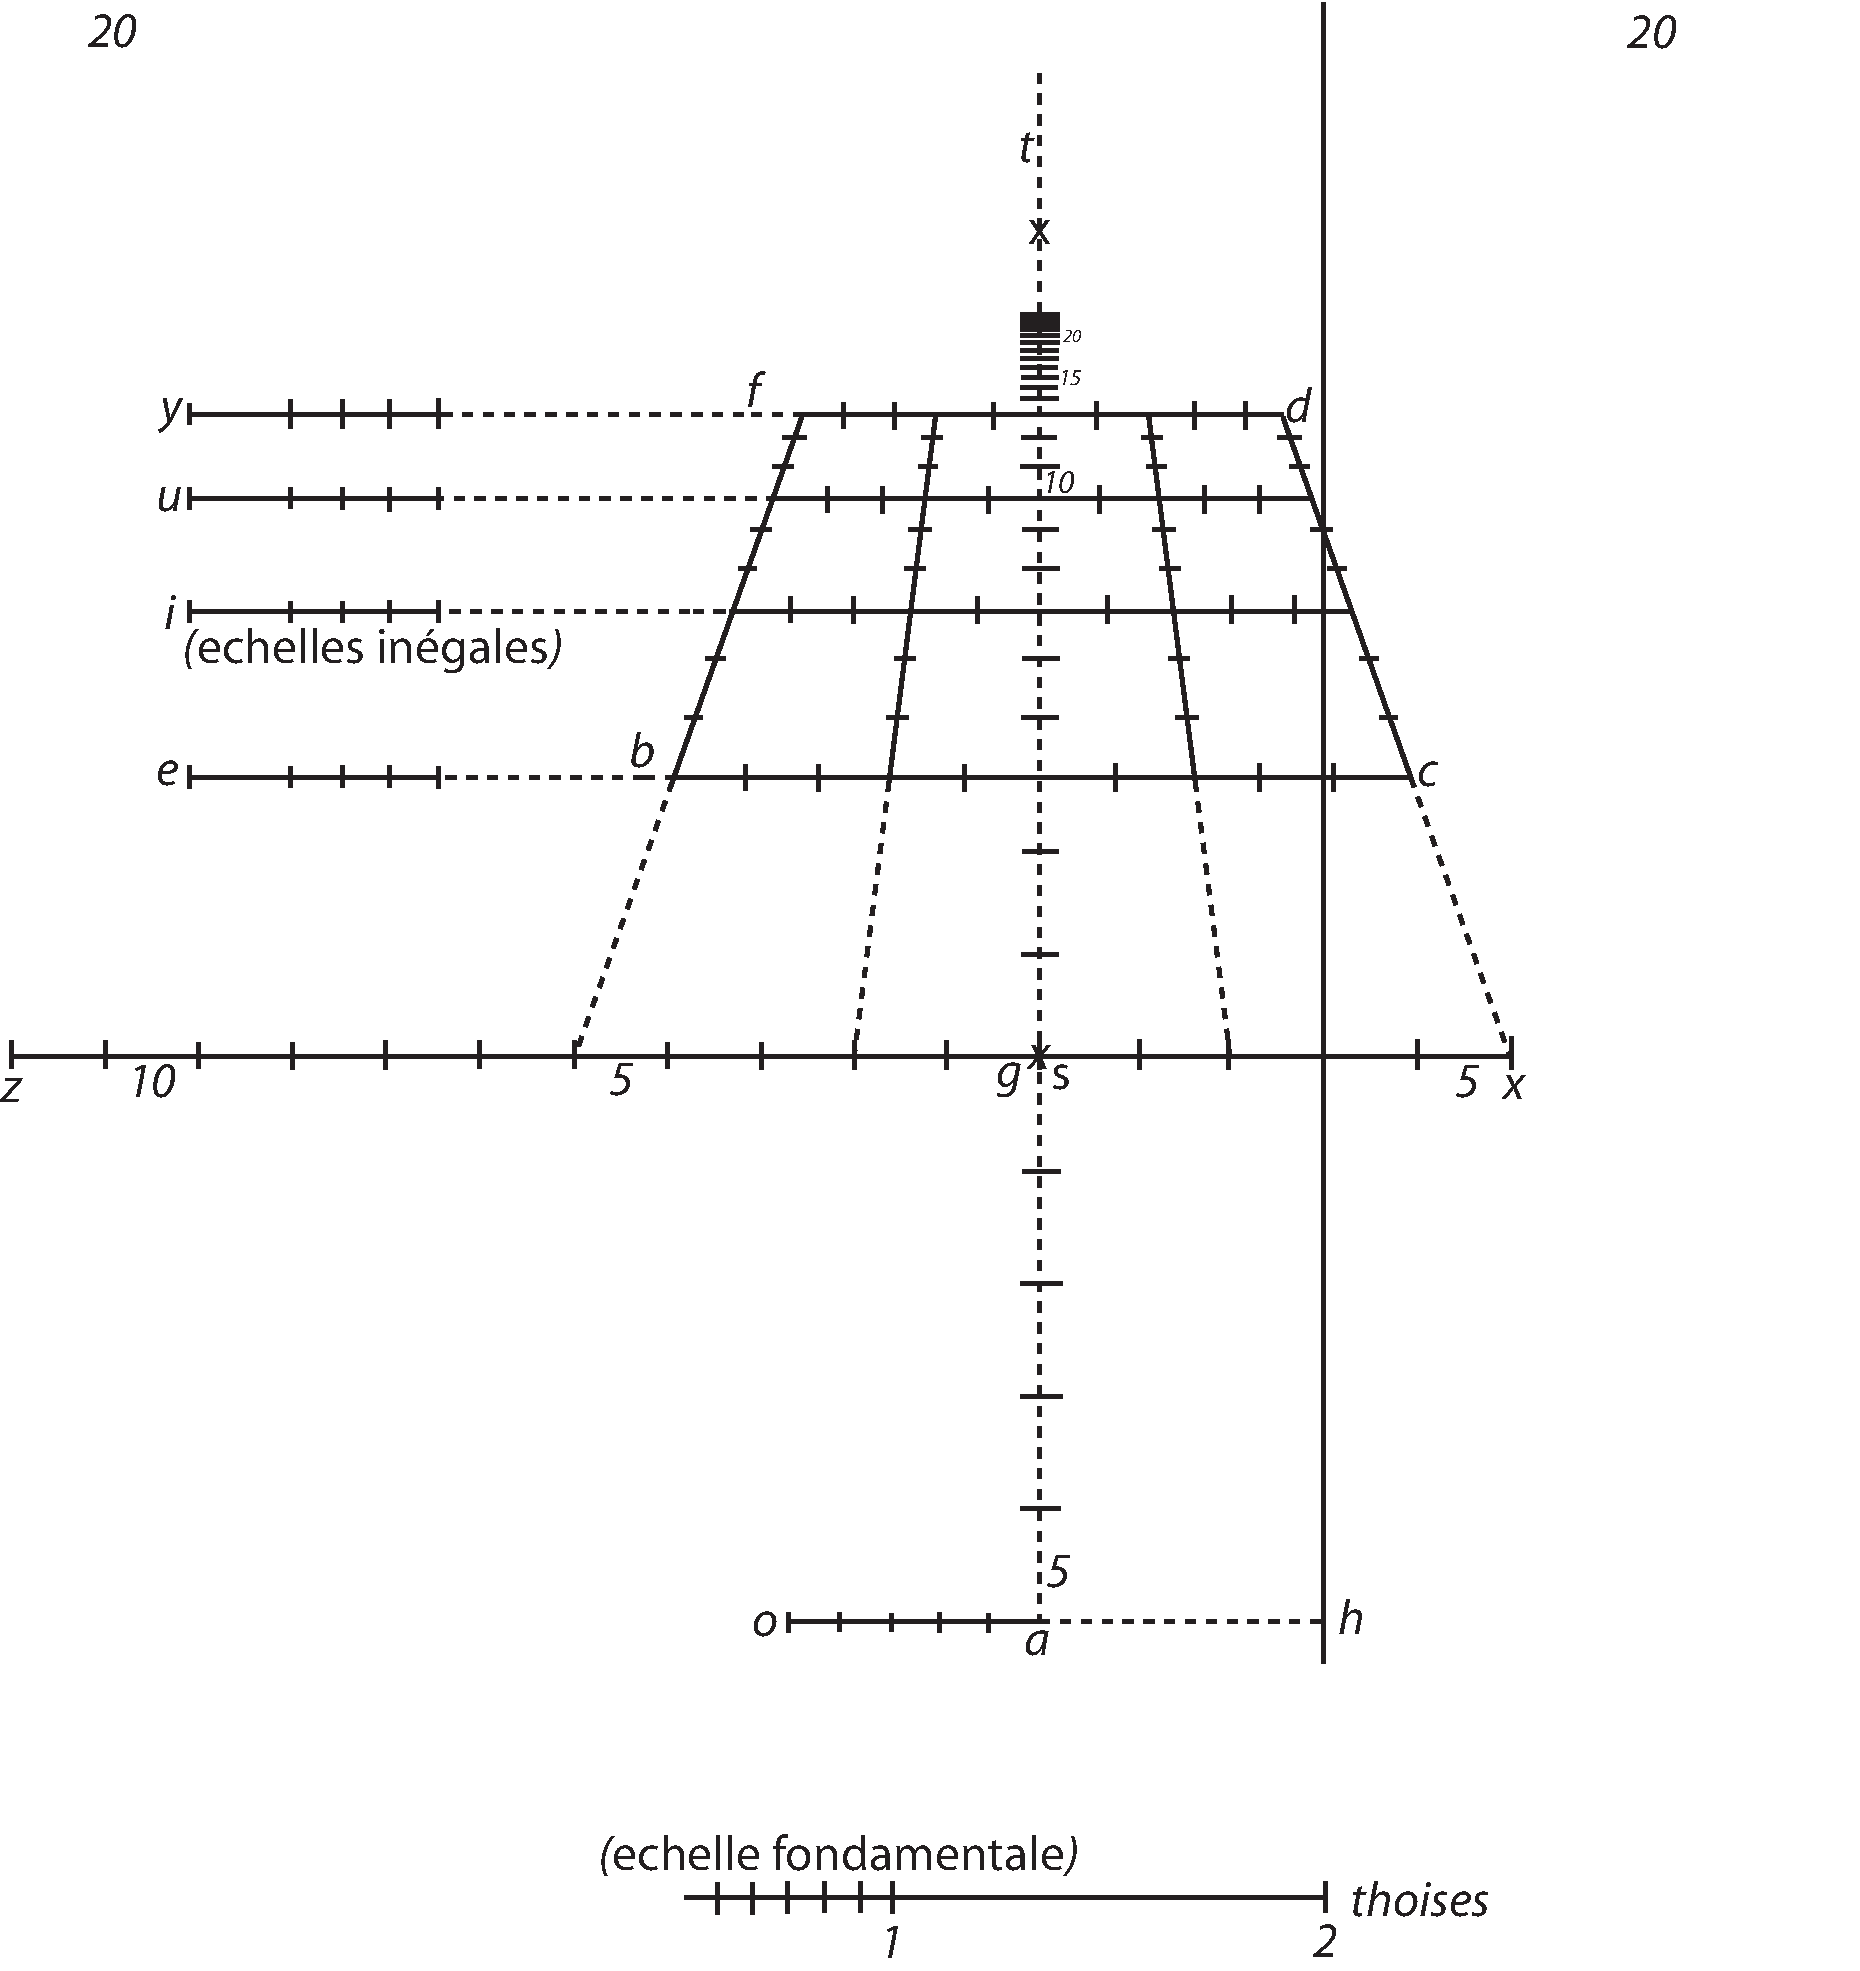
\includegraphics[width=0.9\textwidth]{images/T20-Desargues}
\\\rule[-4mm]{0mm}{10mm}\textit{[Fig. 7]}
\protect\newpage
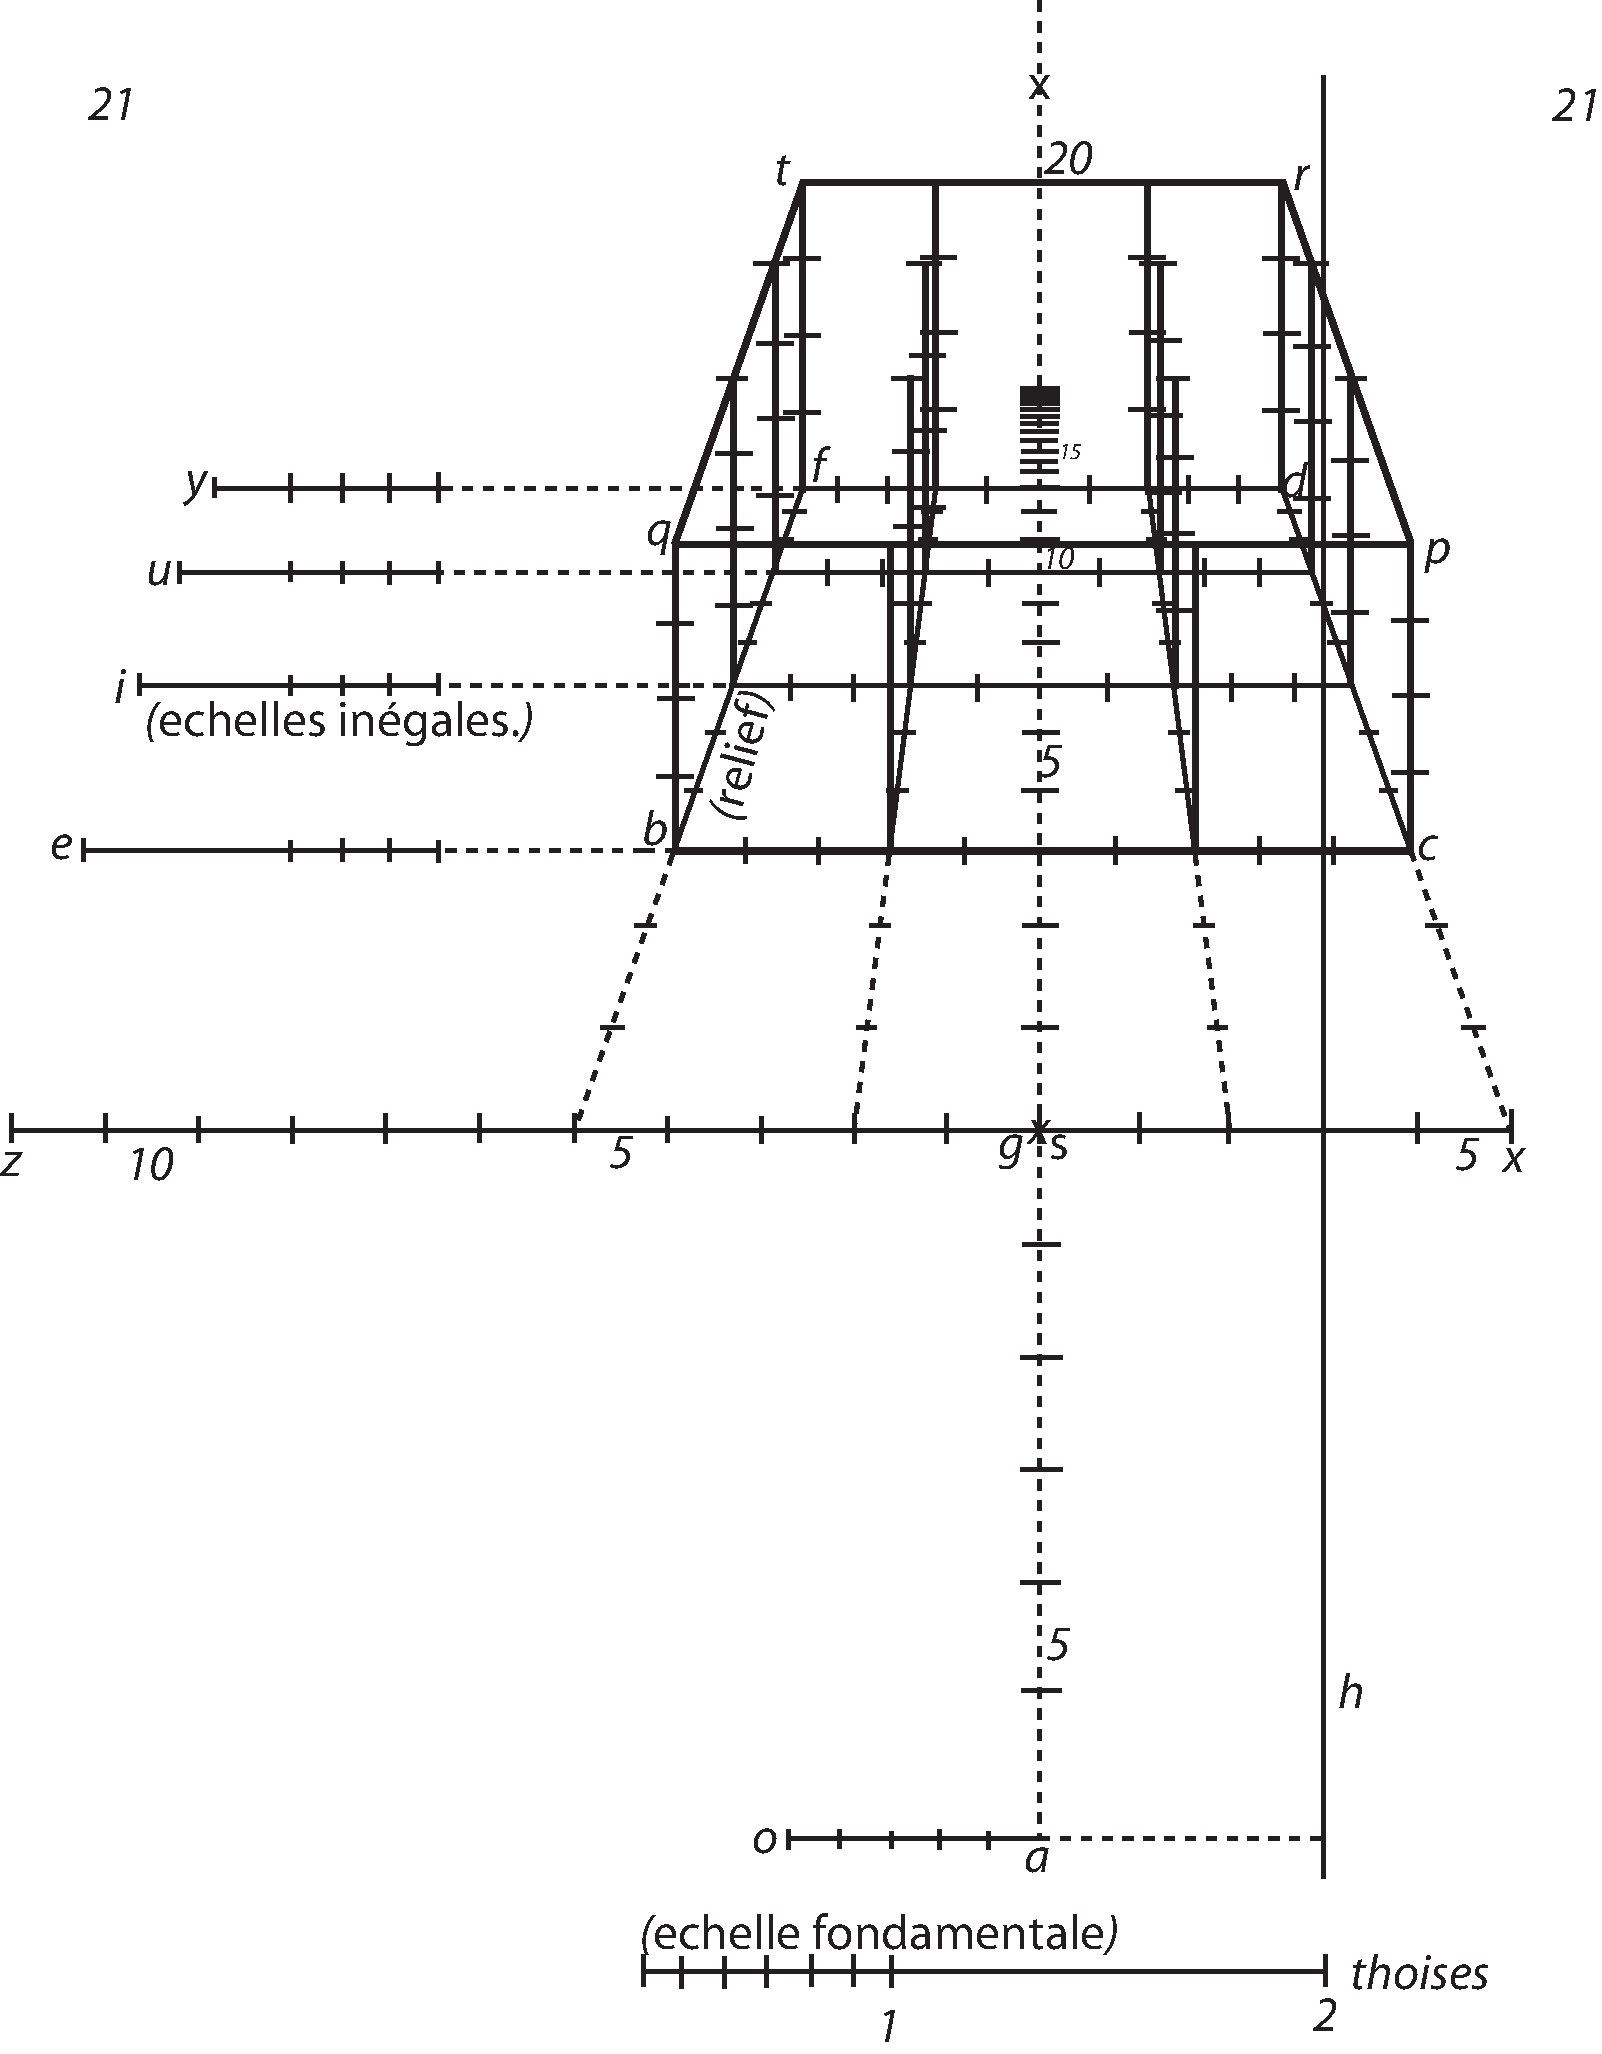
\includegraphics[width=0.9\textwidth]{images/T21-Desargues}
\\\rule[-4mm]{0mm}{10mm}\textit{[Fig. 8]}
\protect\newpage
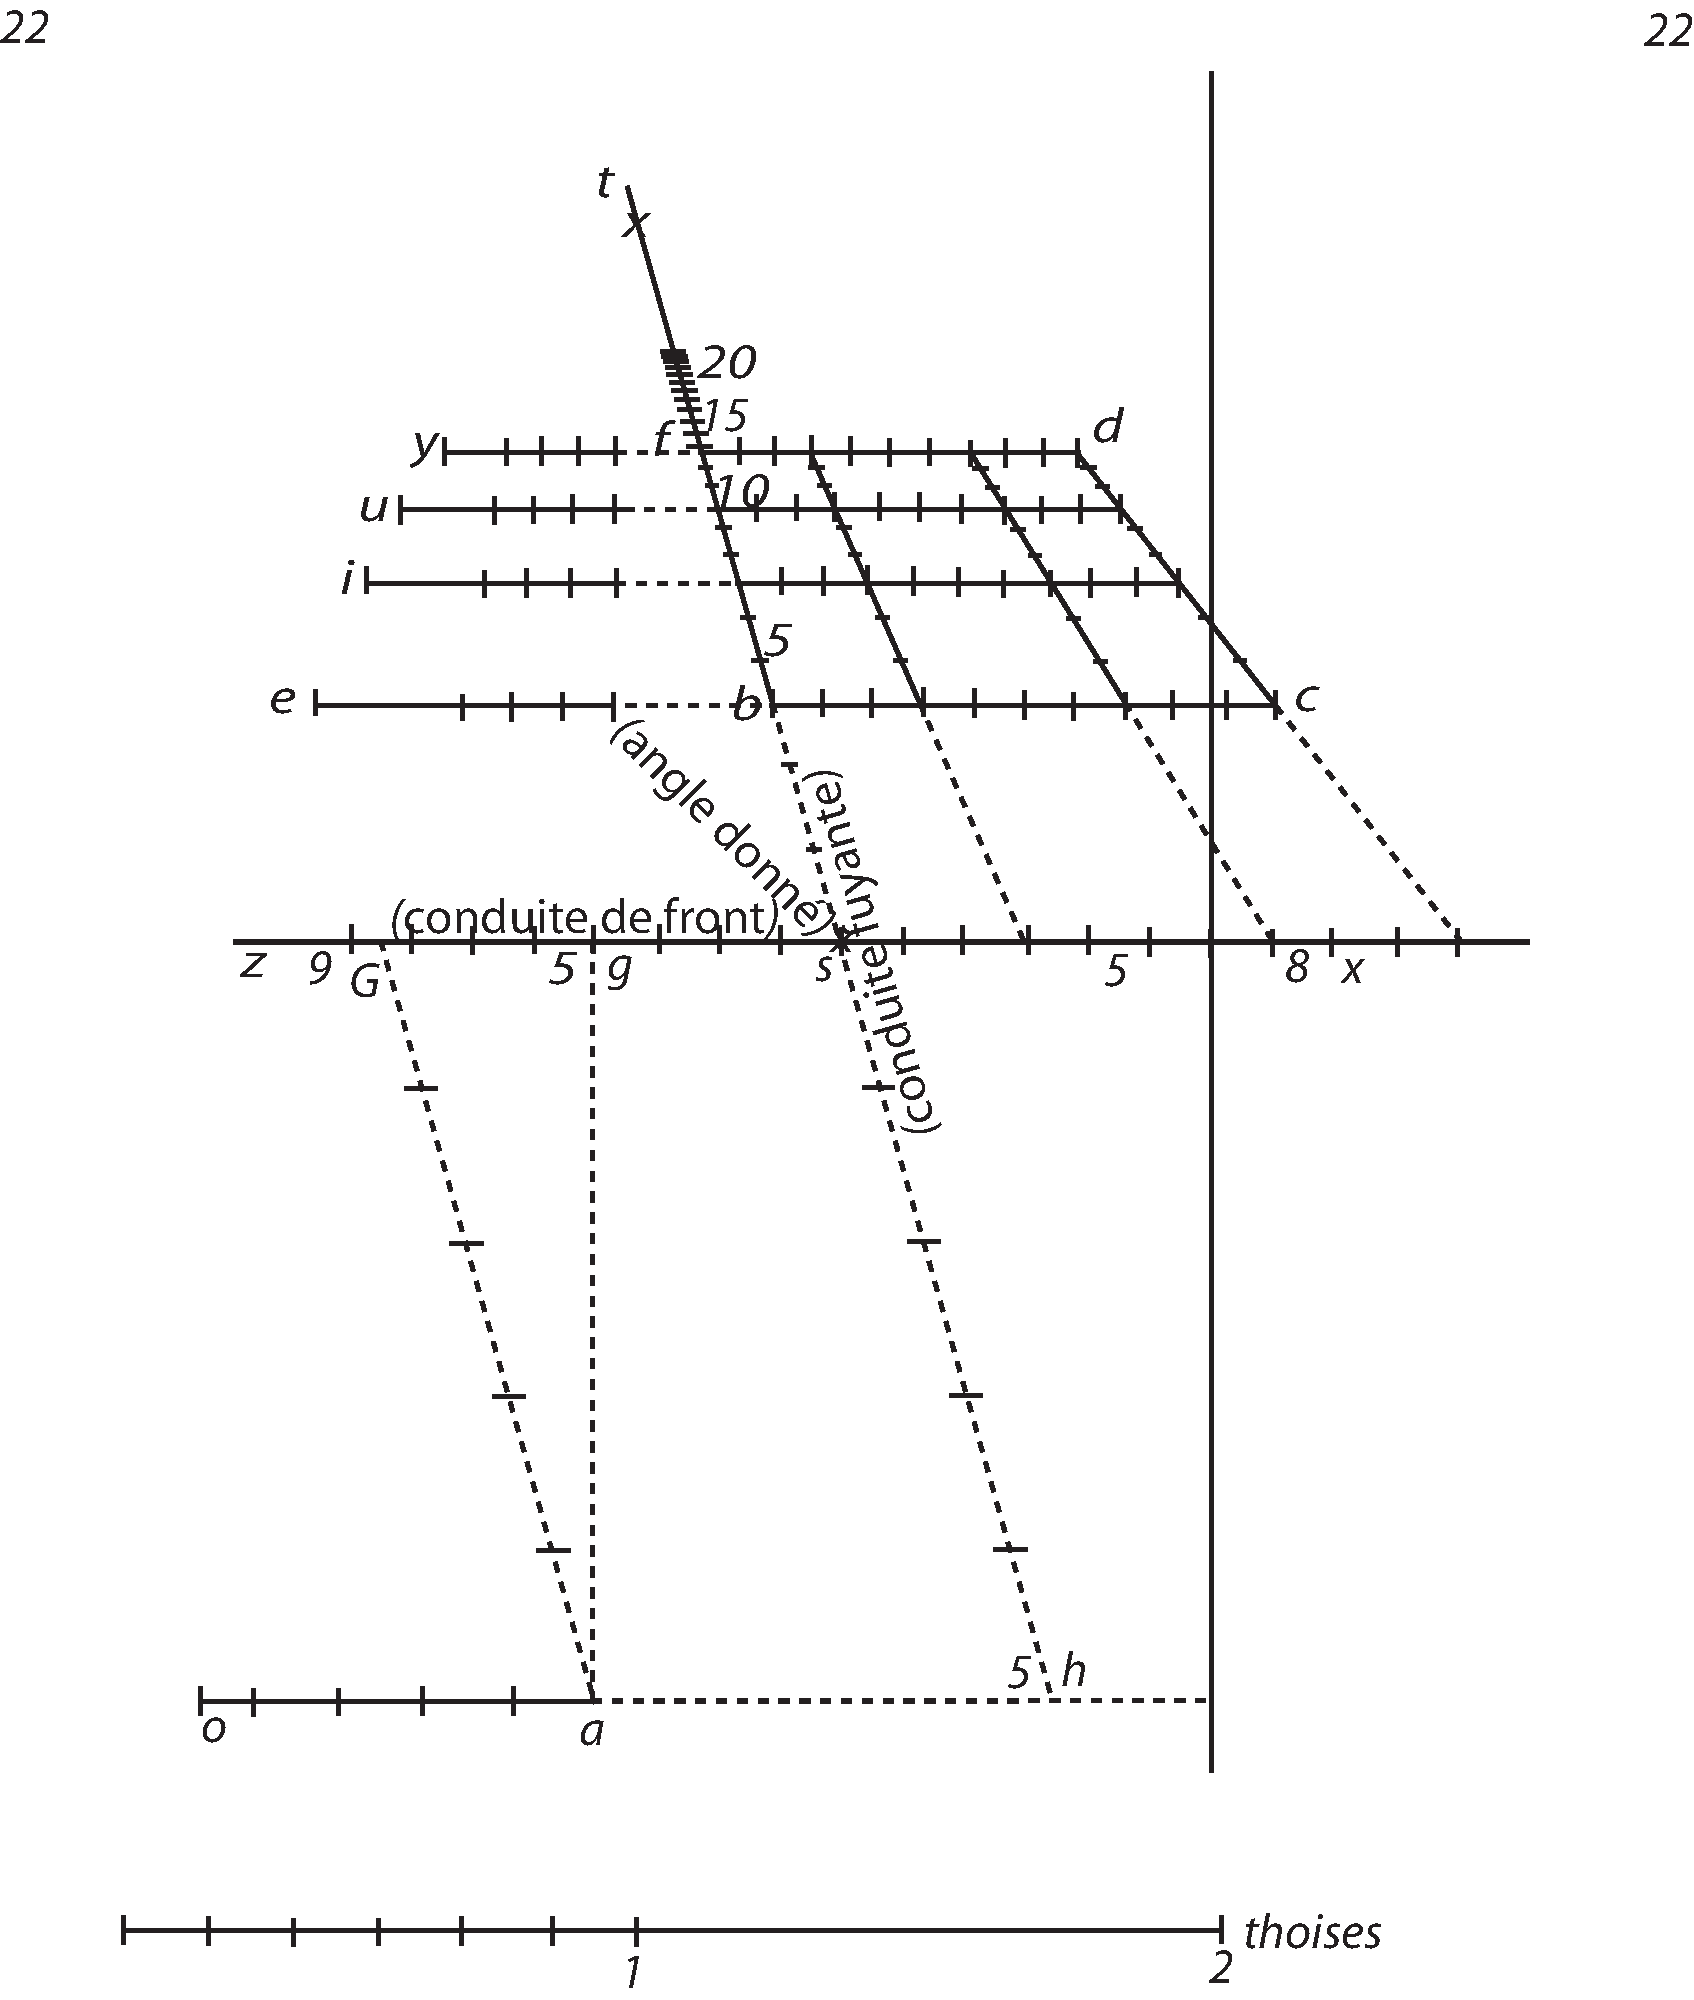
\includegraphics[width=1.0\textwidth]{images/T22-Desargues}
\\\rule[-4mm]{0mm}{10mm}\textit{[Fig. 9]}
\protect\newpage
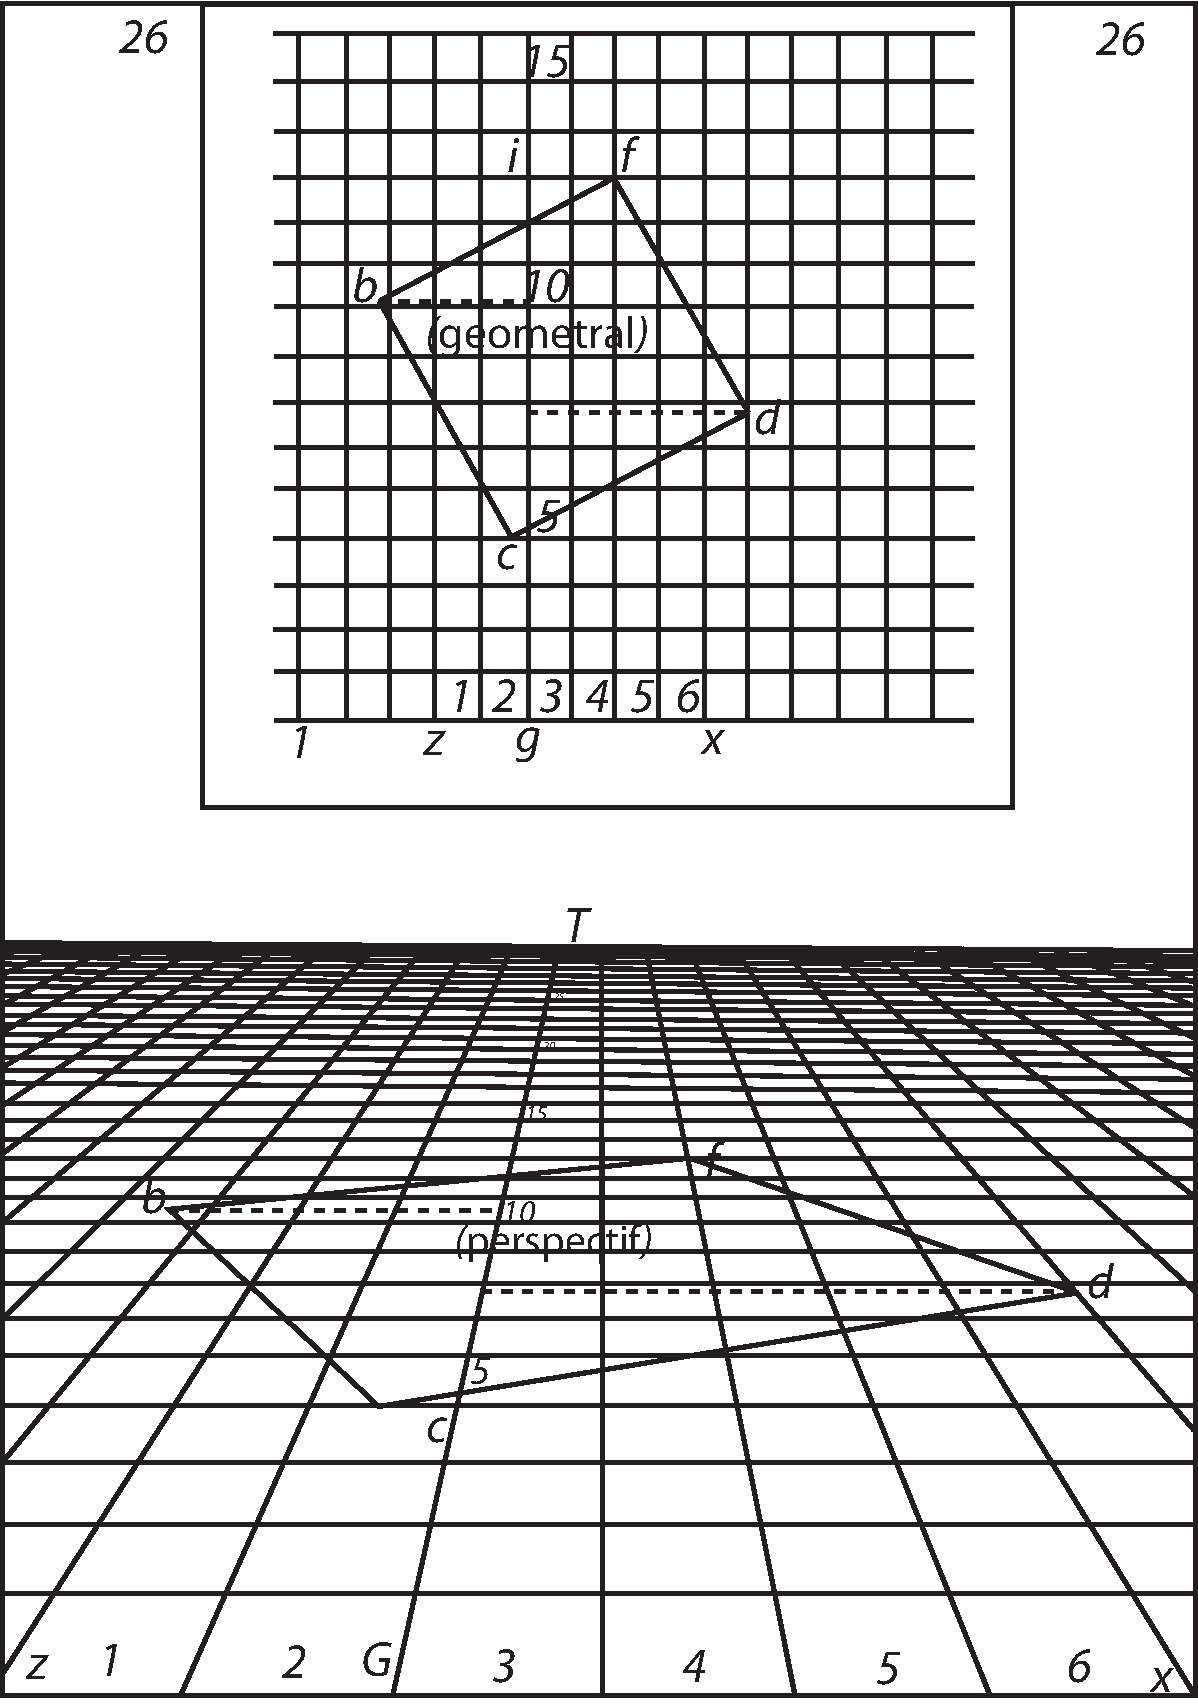
\includegraphics[width=0.75\textwidth]{images/T26-Desargues}
\\\rule[-4mm]{0mm}{10mm}\textit{[Fig. 10]}
\protect\newpage
\pstart [p.~86] [...] en apres tirez au del\`{a} de cette conduite, \`{a} autant de ses pieds loin d'elle, que vous voulez que la hauteur de l'oeil\protect\index{Sachverzeichnis}{oeil} en contienne, vne droite ZCX, qui luy soit paralelle; elle sera celle qu'on nomme communement, \textit{horisontale}, et M. D.\footnote{\textit{Leibniz erg\"{a}nzt} M. D. \textit{zu} Mons. Desargues} ligne du plan de l'oeil\protect\index{Sachverzeichnis}{oeil}\footnote{\textit{Am Rand gestrichen}: la figure est fautive}; Dauantage, menez des deux bouts \textit{q} et \textit{p}, duquel que vous voudrez des pieds de la conduite de front E\textit{l}GV, comme icy par exemple de celuy \textit{4}, au point qu'il vous plaira C, de la ligne horisontale ZCX, deux droites fuyantes \textit{q}C, \textit{p}C; elles vous regleront entr'elles deux, l'inegalit\'{e} continuelle qu'il doit y auoir entre les pieds de front de c\'{e}t exemple; c'est \`{a} dire qu'elles en forment l'eschelle des pieds de front:\footnote{\textit{Leibniz unterstreicht}: l'eschelle [...] front} [...].\pend
\protect\newpage
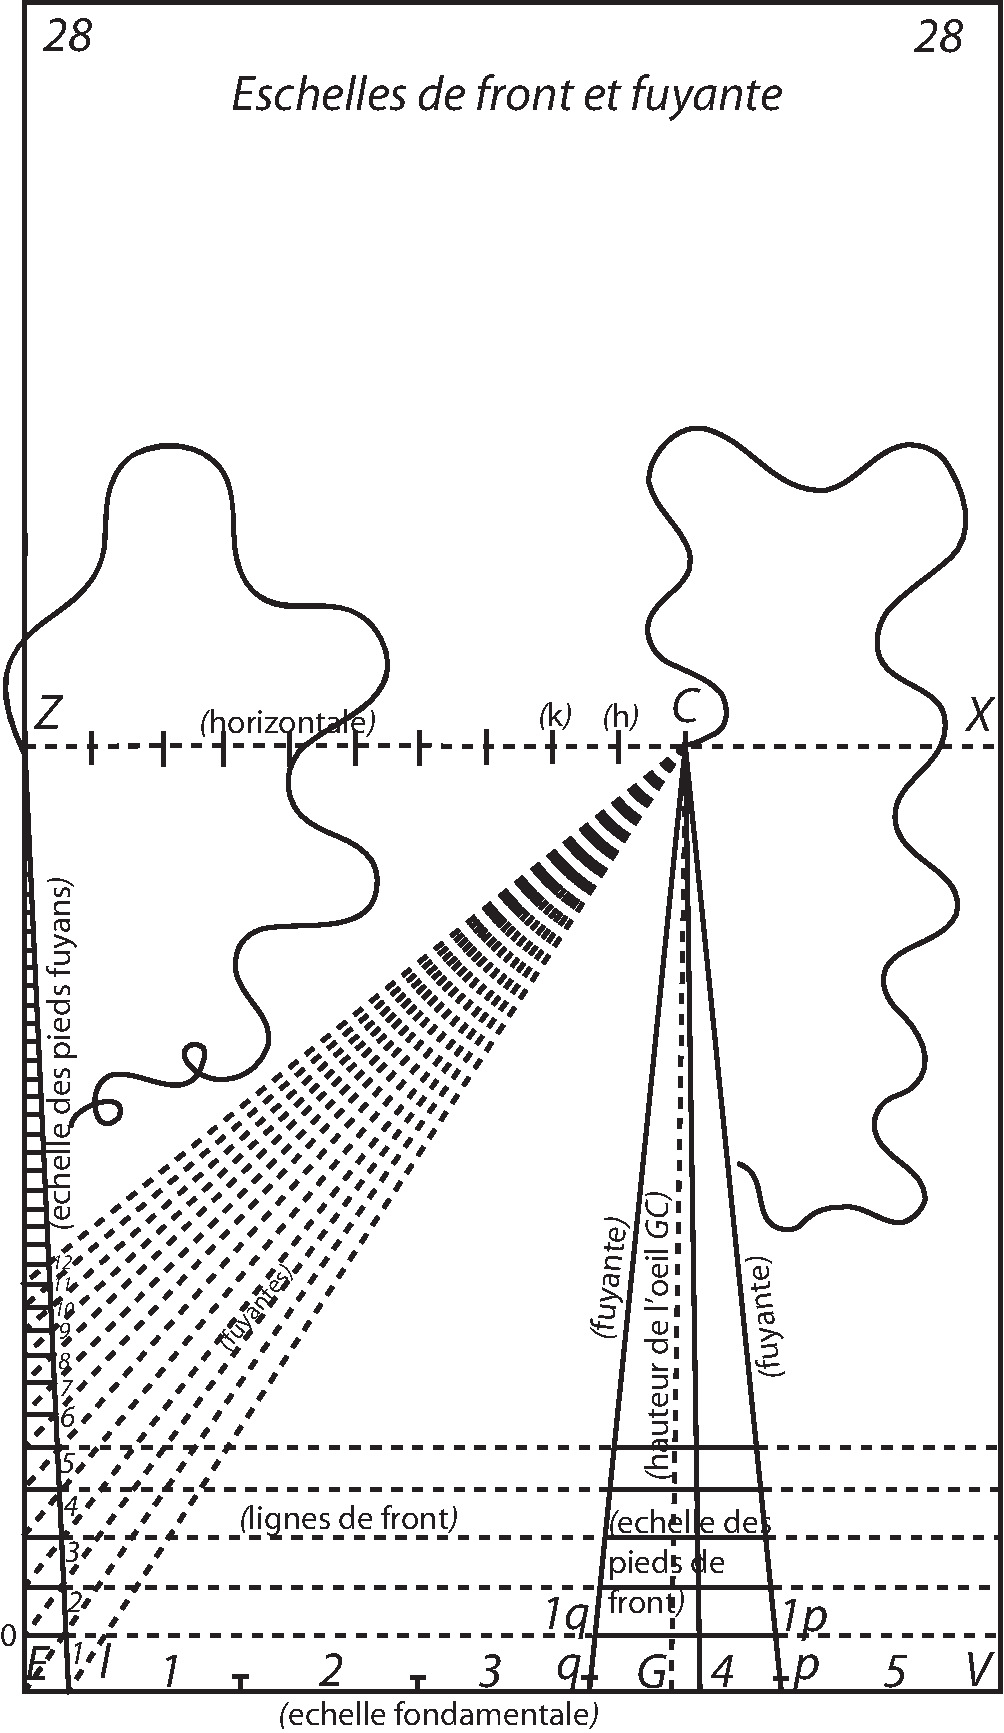
\includegraphics[width=0.6\textwidth]{images/T28-Desargues}\\\rule[-4mm]{0mm}{10mm}\textit{[Fig. 11]}\textsuperscript{10}
\footnoterule
\pstart\noindent\textsuperscript{10}\textit{Unter der \"{U}berschrift}: \textso{Pieds de front} sont les parties des lignes de front; comprises entre deux fuyantes\protect\index{Sachverzeichnis}{\'{e}chelle!fuyante} men\'{e}es des deux bouts \textit{q}, \textit{p} d'un pied de
\\
\footnoterule\\
l'echelle\protect\index{Sachverzeichnis}{\'{e}chelle} fondamentale \textit{EV} \`{a} un point \textit{C} de la ligne horizontale; \textit{ZX}.\textso{ L'echelle}\protect\index{Sachverzeichnis}{\'{e}chelle!de front} de front est la suite des pieds de front compris entre deux m�mes fuyantes. Prenez dans l'echelle\protect\index{Sachverzeichnis}{\'{e}chelle} fondamentale, une droite \textit{EL}, qui est \`{a} un pied de l'echelle\protect\index{Sachverzeichnis}{\'{e}chelle} fondamentale \textit{qp} comme \textit{CZ} prise dans l'horizontale depuis le point \textit{C}, est \`{a} la distance de la station \`{a} la conduite de front. Men\'{e}s \textit{EZ}, \textit{lZ } les parties des lignes de front, comprises entre les deux fuyantes \textit{EZ}, \textit{lZ} seront les pieds fuyans et leur suite sera l'echelle\protect\index{Sachverzeichnis}{\'{e}chelle} des pieds fuyans.\\ \textit{In der Mitte unter der Geraden}: \textit{ZX}: \textit{ch}, \textit{hk}, etc. \'{e}gal \`{a} \textit{El}\\ \textit{Links unter der Geraden}: \textit{ZX}: \textit{CZ} est autant de fois \textit{El} que la distance de la station \`{a} la conduite de front, a des pieds de long.\\ \textit{Unter der Zeichnung links}: \textit{El}\textso{ pied fuyans fondamental.} \textit{NB}\\ \textit{Unter der Zeichnung}: Suppose \textit{ZE} parallele \`{a} \textit{CG} il se demontre que \textit{EO} est egale \`{a} \textit{1q1p} car \textit{EO} : \textit{ZO} :: \textit{El} : \textit{GE} :: \textit{qp} : \textit{CZ} :: \textit{1q1p} : \textit{ZO}. La figure est mal faite, car \textit{CZ} deuuroit estre \`{a} \textit{CG} comme \textit{El} \`{a} \textit{qp}, et les deux premiers estans faits quasi egaux. Les derniers le deuuroient estre \edtext{aussi. \selectlanguage{latin} }{\lemma{aussi.}\Afootnote{\textbar\ supposant \textit{ZE} et \textit{CG} item \textit{CZ} et \textit{lE} paralleles et egales \textit{ gestr.}\ \textbar\ \ \ \ \textit{L}}}\\ \textit{Unter der Zeichnung rechts}: \textso{pied de front fondamental} NB, et \textso{pied geometral} NB sont une m�me chose \textit{qp}.\\ \textit{Neben der Zeichnung rechts am Rand}: \textit{CG} hauteur de l'oeil \textit{qp} pied \edtext{geometral \textit{El}}{\lemma{geometral}\Afootnote{ \textbar\ egal si vous voul\'{e}s \`{a} \textit{pq} \textit{ gestr.}\ \textbar\ \textit{El}\ \textit{L}\hspace{6cm}}} pris \`{a} discretion\\
\protect\begin{tabular}{l}$CZ:CG::EL:qp$\\$EG\hspace{9pt}CZ$\protect\end{tabular}\\\textit{EO} : \textit{O1} :: \textit{EZ} : \textit{CZ} :: \textit{qp} : \textit{El}\textit{ZO} : \textit{O1} :: \textit{ZE} : \textit{El} \\\rule[-4mm]{0mm}{10mm} $\protect\overbrace{\frac{ZE\cdot EI}{qp}}^{E0\cdot CZ}\protect\overbrace{ZE - E0}^{\sqcap\hspace{5pt} Z0\hspace{5pt}EI}$ \\seu \textit{ZO} : \textit{EO} :: \textit{GE} : \textit{El}. Ergo $\displaystyle 1\sqcap\frac{CG}{E0} - \frac{CG}{qp}$ seu $\displaystyle E0\; \sqcap \frac{CG\cdot qp}{CG+qp}$ \\itaque \textit{EO} prodit eadem, qualiscunque sumatur \textit{El} $\displaystyle CZ \sqcap \frac{CG \cdot El}{qp}$\rule[-4mm]{0mm}{10mm} 
\pend \addtocounter{footnote}{1}
\protect\newpage
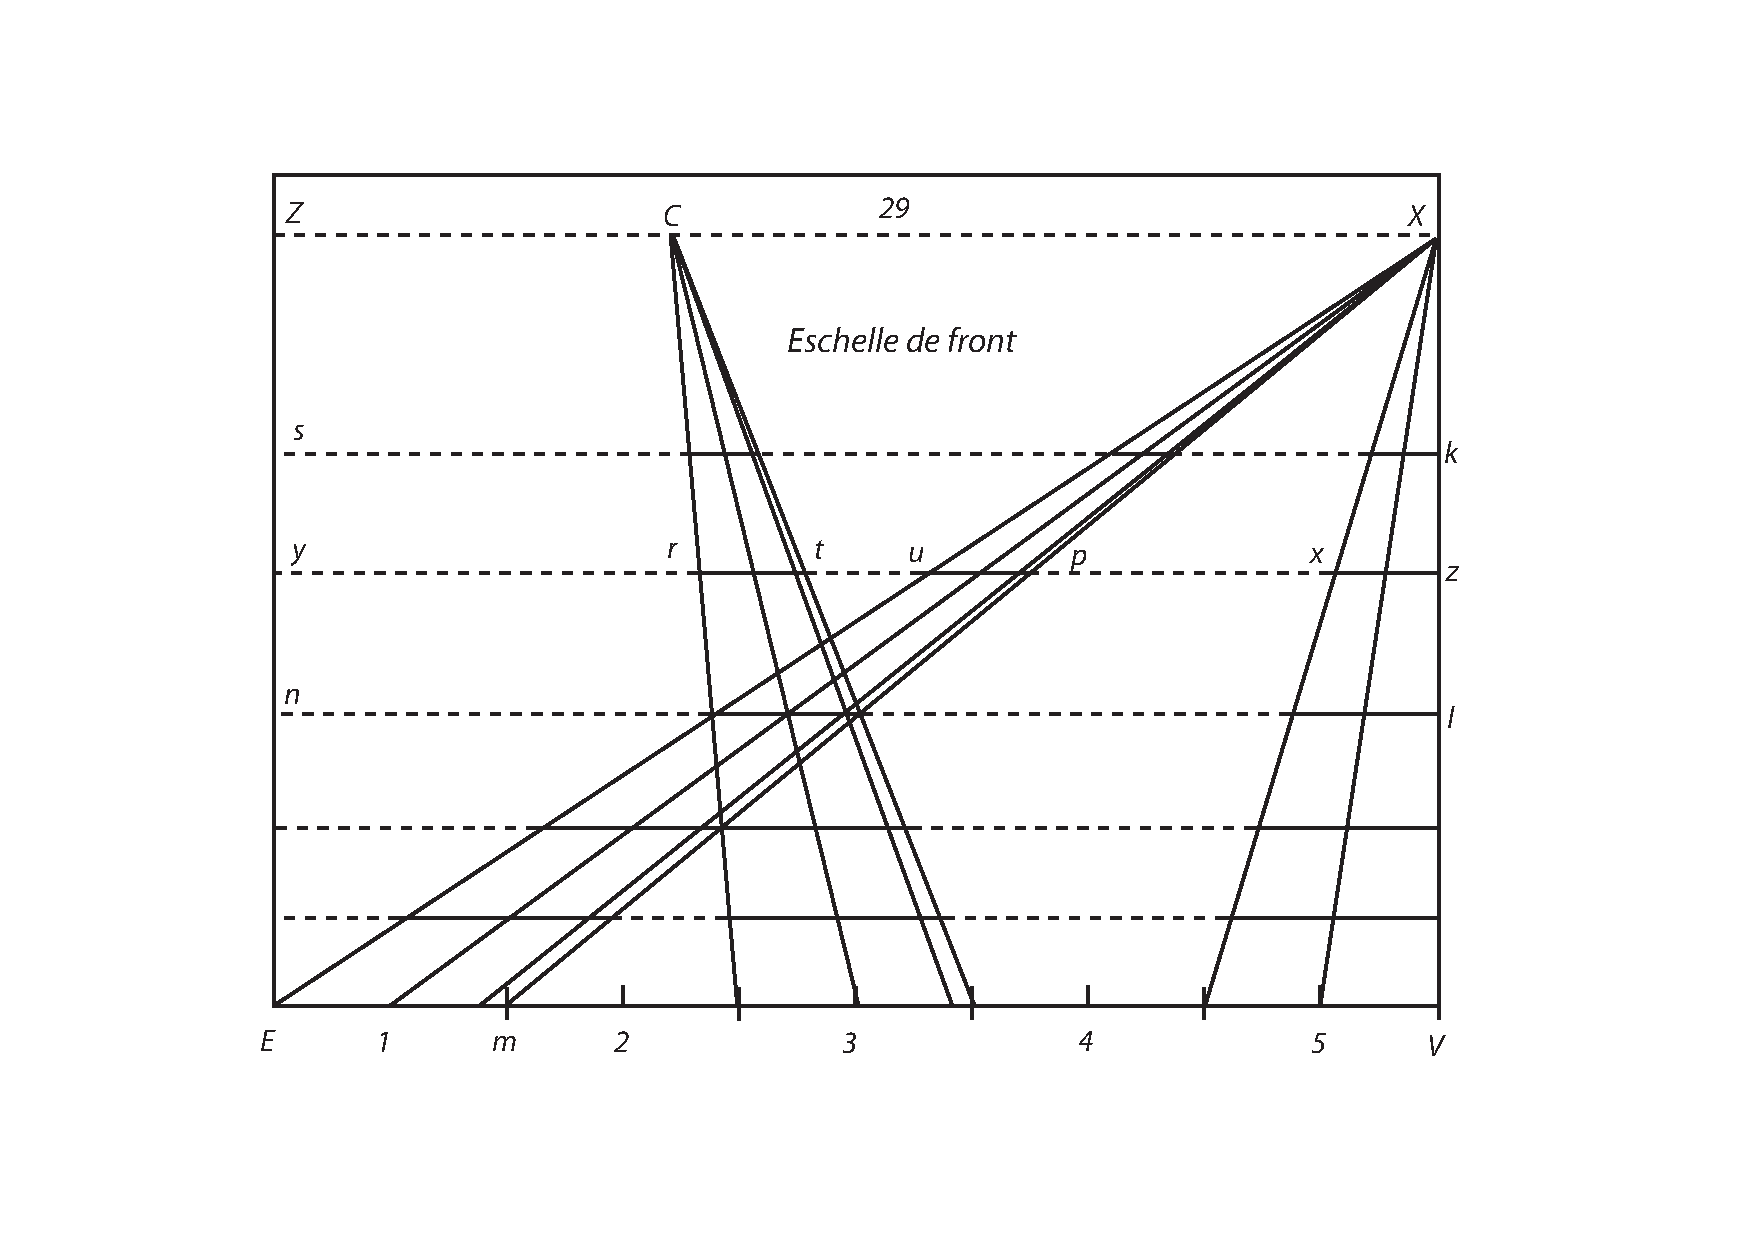
\includegraphics[width=1\textwidth]{images/T29-Desargues_87_a}
\\\textit{[Fig. 12a]}
\footnote{\textit{\"{U}ber der Strecke tu}: \textit{rt} \'{e}gal \`{a} \textit{up} ou \`{a} \textit{xz}}
\end{center}
\begin{center}
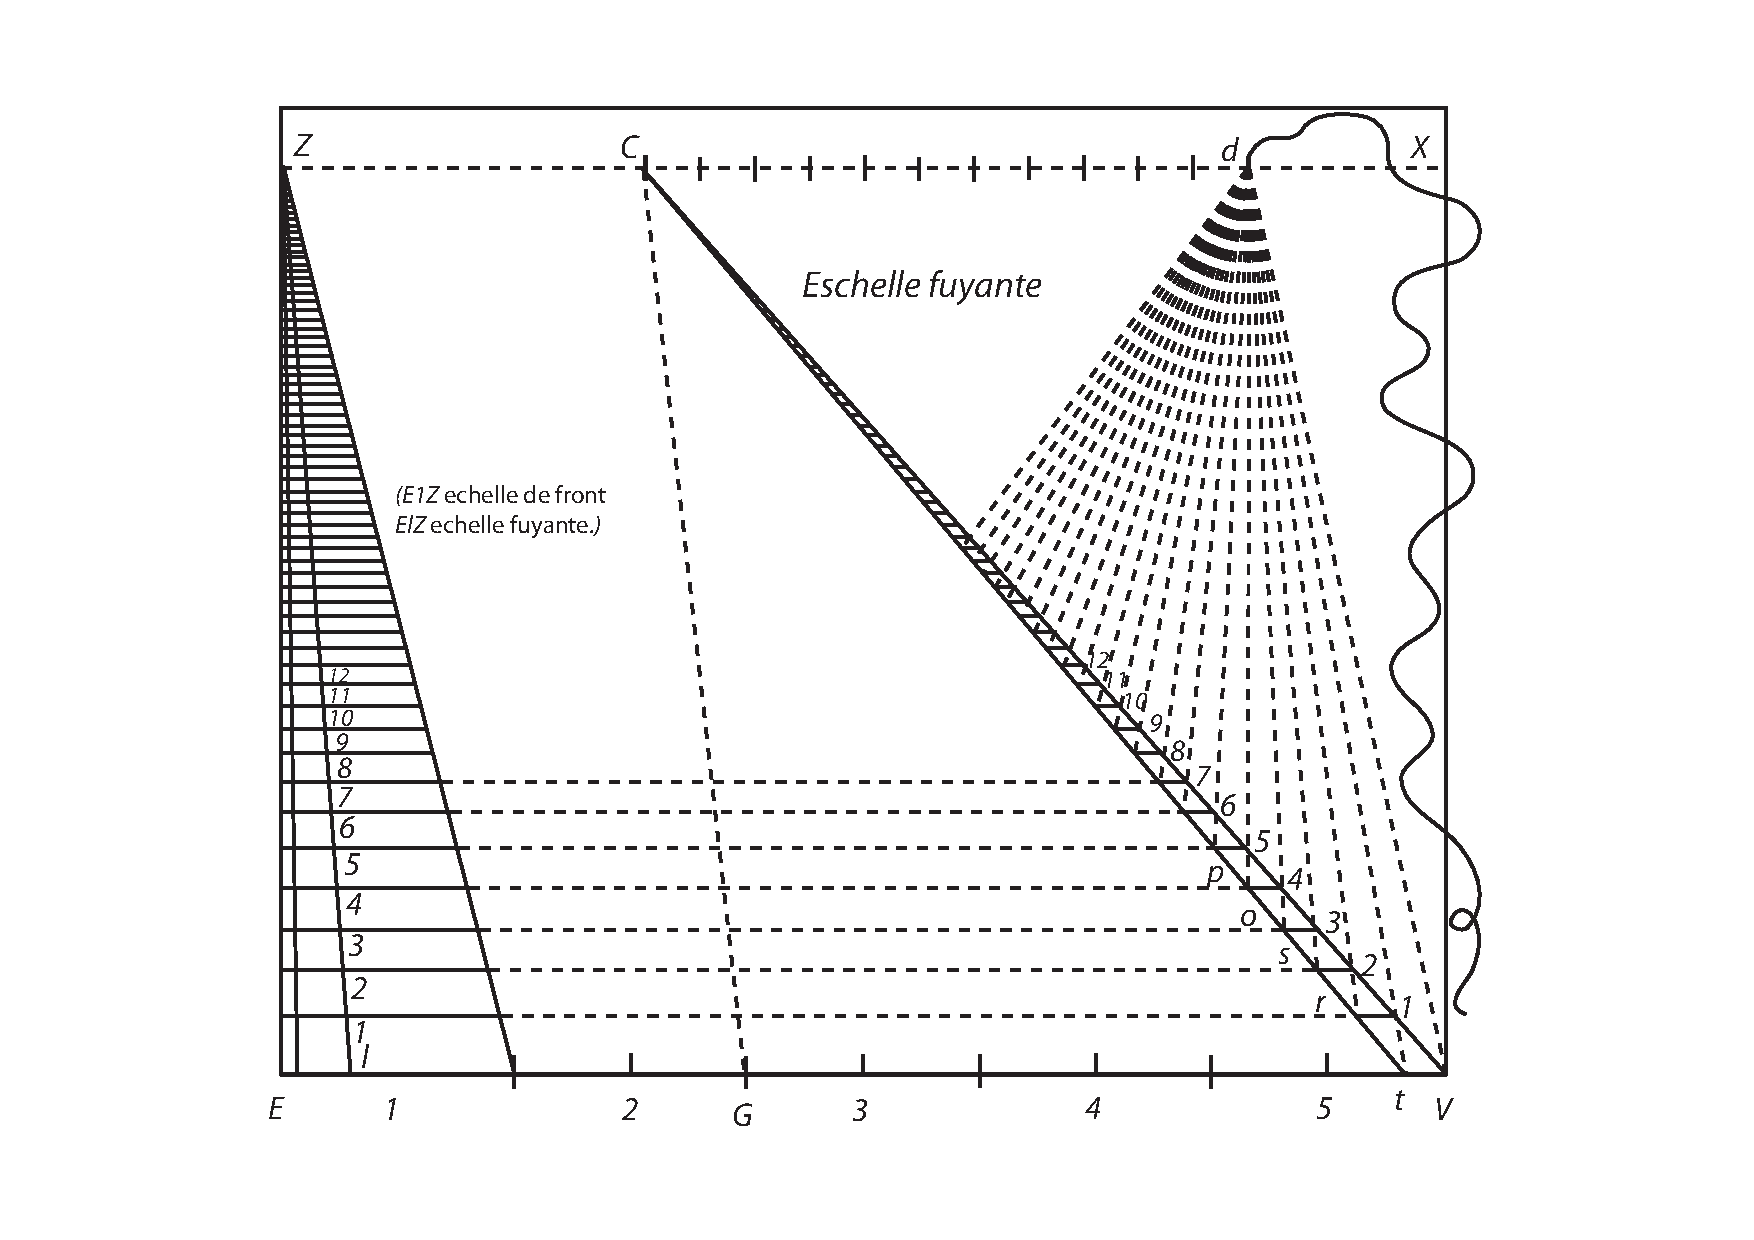
\includegraphics[width=1\textwidth]{images/T29-Desargues_87_b}
\\\textit{[Fig. 12b]}
\footnote{\textit{Links unter der Geraden ZX}: \textit{cd} \`{a} \textit{Vt} ou \`{a} \textit{dh} comme la distance de la station \`{a} la conduite de front est \`{a} un pied \textit{E1}. \\ \textit{Rechts unter der Geraden }\textit{ZX}: \textit{dh} \'{e}gal \`{a} \textit{Vt} \\ \textit{Oben links neben der Geraden CV}: \protect\begin{tabular}{c} dp\\do\protect\end{tabular} coupe \textit{CV} en \protect\begin{tabular}{c} 5\\4\protect\end{tabular}\rule[-4mm]{0mm}{10mm}  \\ \textit{Im unteren Teil der Abbildung in der Mitte links neben der Geraden CV}: \textit{E1Z} echelle de front\protect\index{Sachverzeichnis}{\'{e}chelle!de front} \textit{ElZ} echelle fuyante\protect\index{Sachverzeichnis}{\'{e}chelle!fuyante}.}
\end{center}